\section{Daten}\label{chap:Daten} 
Diese Thesis konzentriert sich auf zwei Datensätze, die medizinische Bilder enthalten. Der COVIDx CXR-4 Datensatz umfasst Bilder von Patienten mit und ohne COVID-19, während der Brain Tumor Datensatz Bilder von Hirntumoren sowie gesunde Kontrollbilder beinhaltet.

% Gender? -> Patienten -> Personen : Patient*innen

\subsection{COVIDx CXR-4} \label{chap:COVIDx CXR-4}
COVID-19, verursacht durch das Coronavirus SARS-CoV-2, ist eine hochansteckende Atemwegserkrankung. Sie wurde erstmals Ende 2019 identifiziert. Die Symptome reichen von mildem Husten und Fieber bis hin zu schweren Verläufen wie Lungenentzündung und akutem Atemnotsyndrom. Aufgrund der hohen Übertragbarkeit und der potenziell schweren Verläufe hatte die Pandemie weitreichende Auswirkungen auf das globale Gesundheitssystem, die Wirtschaft und das tägliche Leben der Menschen.

\textbf{COVIDx CXR-4} \cite{wu_covidx_2023} ist ein öffentlicher Datensatz für die COVID-19 Diagnostik mit Röntgenbildern, der 84'818 Bilder von 45'342 Patienten enthält. COVIDx CXR-4 ist nach Kenntnisstand der Autoren der grösste und vielfältigste öffentlich verfügbare COVID-19 Datensatz für Röntgenbilder und soll die Forschung unterstützen, um Kliniker im Kampf gegen COVID-19 zu helfen.

Patienten mit einem negativen Befund erhalten das Klassenlabel Null, bei einem positiven Befund das Klassenlabel Eins. Die Röntgenbilder beschränken sich auf den Brustkorb der jeweiligen Personen.

\begin{figure}[H]
    \centering
    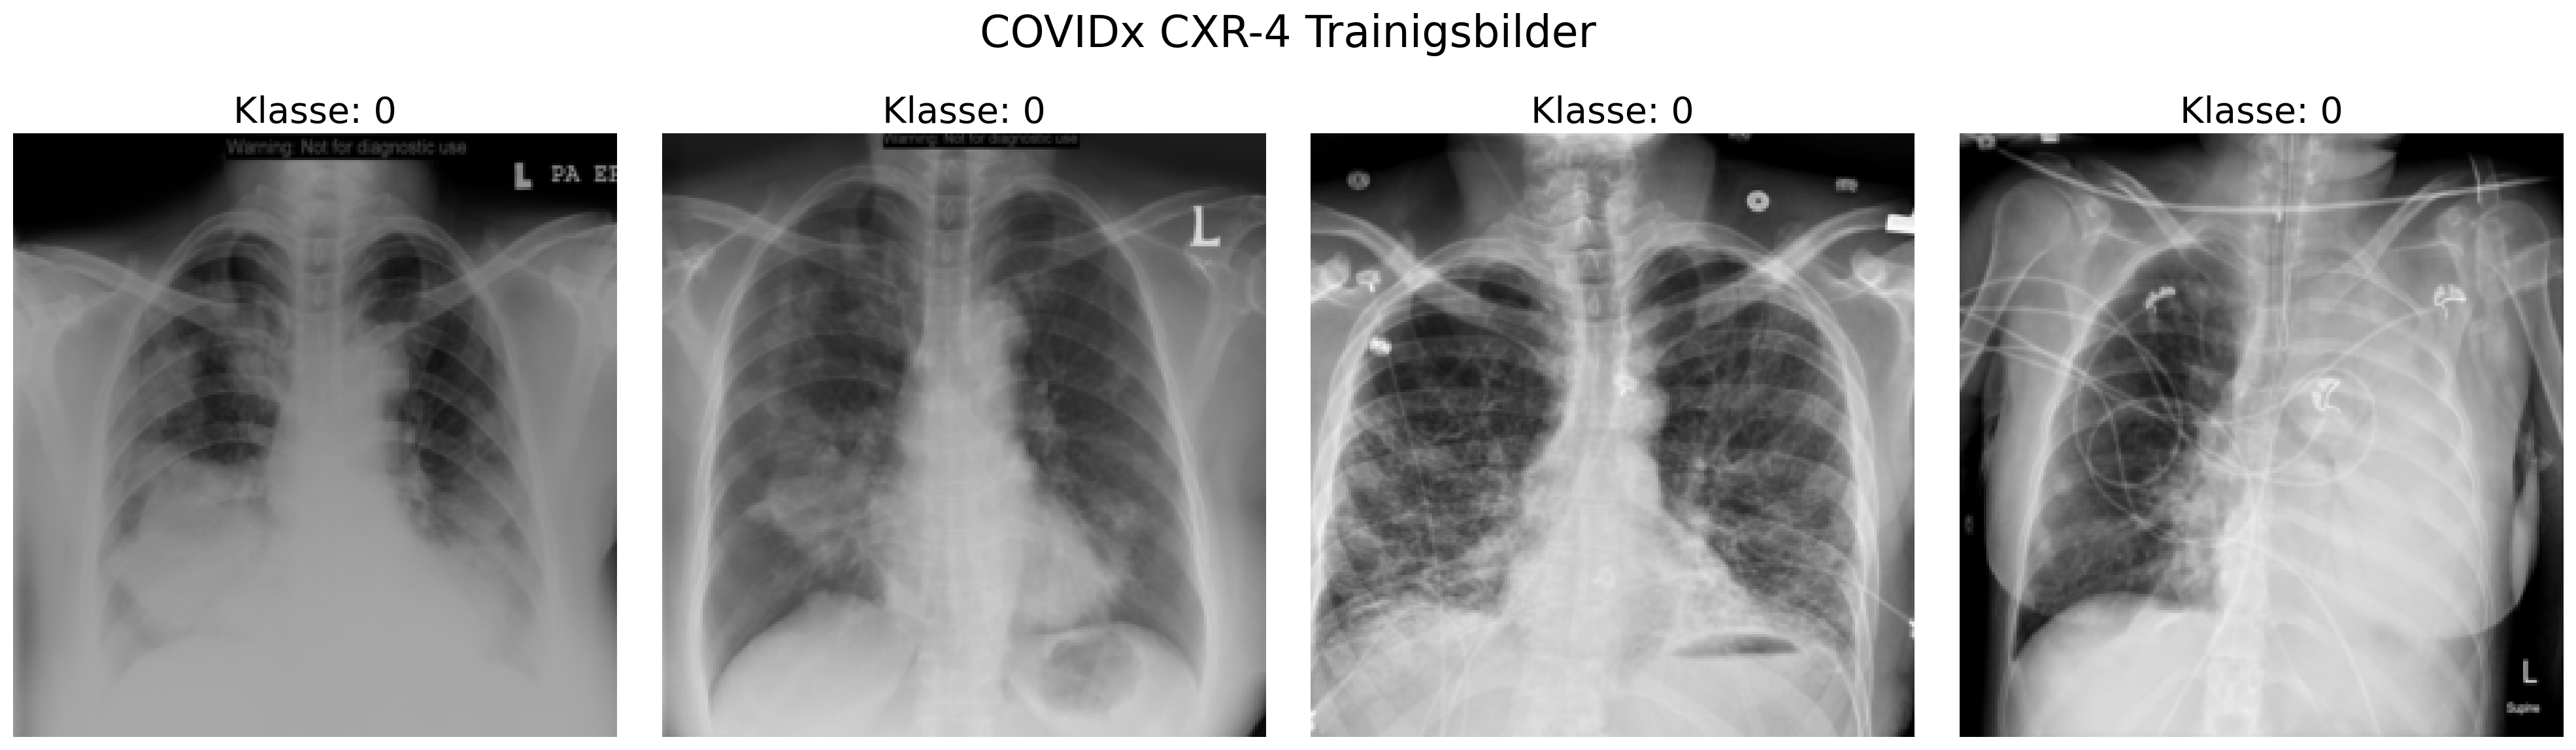
\includegraphics[width=\linewidth]{01-images/03-data/covid19-klasse0.png}
    \caption{Beispiele von Patienten mit einem negativen COVID-19 Befund}
    \label{fig:covid19-beispiele-klasse0-negativ}
\end{figure}

\begin{figure}[H]
    \centering
    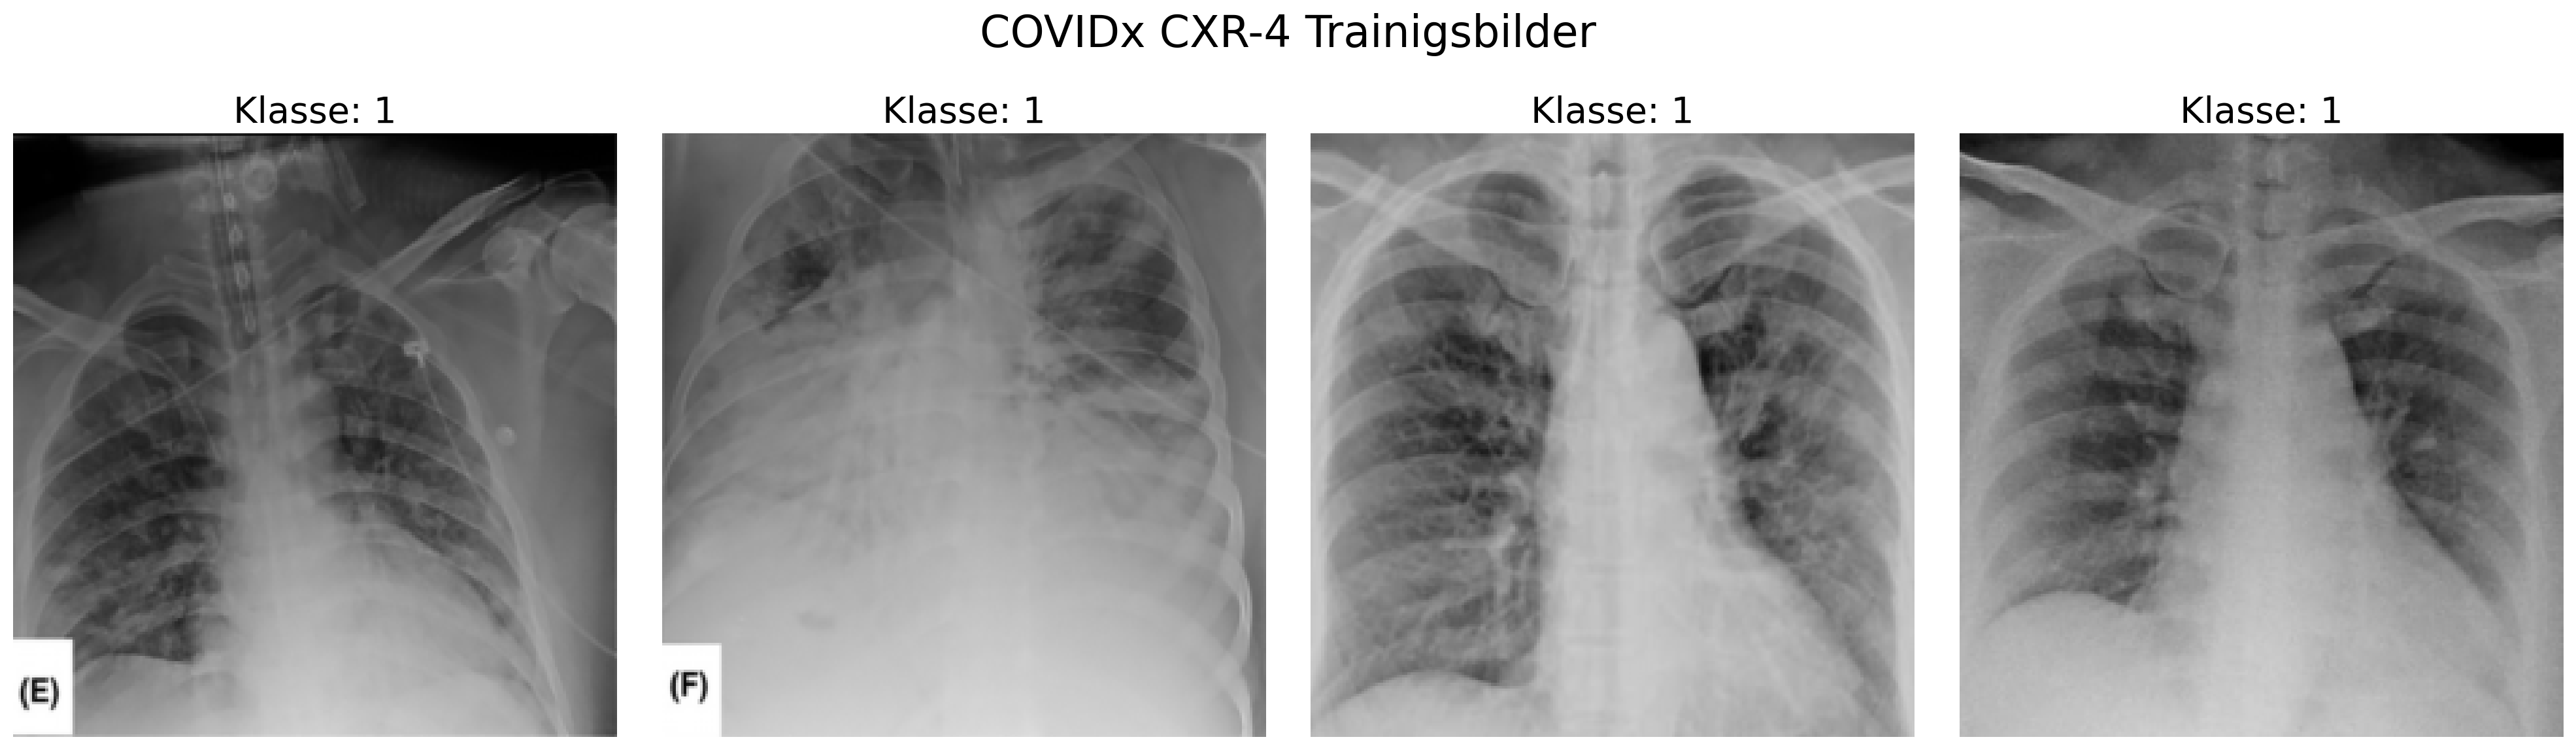
\includegraphics[width=\linewidth]{01-images/03-data/covid19-klasse1.png}
    \caption{Beispiele von Patienten mit einem positiven COVID-19 Befund}
    \label{fig:covid19-beispiele-klasse1-positiv}
\end{figure}

\subsubsection{Datenpartitionierung} \label{chap:COVID19-Partition}
Die Datenpartitionierung ist bereits durch die Struktur vorgegeben. Die Klassenverteilung von positiven und negativen Labels für die Validierungs- und Testdatensätze ist nahezu gleich verteilt, mit einem Verhältnis von 50\% positiven zu 50\% negativen Fällen.

\begin{table}[h]
    \centering
    \begin{tabular}{@{}cccccc@{}}
        \toprule
        Partition & \multicolumn{2}{c}{Anzahl Bilder} & \multicolumn{2}{c}{Klassenverteilung} & Positiv-Verhältnis\\ 
        \cmidrule(lr){2-3} \cmidrule(lr){4-5} 
                  & Absolut & Relativ & Positiv & Negativ & \\ 
        \midrule
        Train      & 67863 & 0.8001 & 57199 & 10664 & 0.8429 \\
        Validation & 8473  & 0.0999 & 4241  & 4232  & 0.5005 \\
        Test       & 8482  & 0.1000 & 4241  & 4241  & 0.5000 \\ 
        \bottomrule
    \end{tabular}
    \caption{Datenpartitionierung vom COVIDx CXR-4 Datensatz}
    \label{tab:covid19-klassenverteilung}
\end{table}

\subsubsection{Datenexploration} \label{chap:COVID19-eda}
Die Histogramme in den Abbildungen \ref{fig:covid19-klasse0-hist} und \ref{fig:covid19-klasse1-hist} zeigen die Pixelverteilung der Röntgenbilder von Patienten mit positiven und negativen Befunden aus Abbildung \ref{fig:covid19-beispiele-klasse0-negativ} und \ref{fig:covid19-beispiele-klasse1-positiv}. Jedes Histogramm stellt die Intensitätsverteilung der Pixelwerte in den jeweiligen Röntgenaufnahmen dar. Auf der x-Achse jedes Histogramms wird die Grauwertintensität von 0 bis 255 dargestellt, während die y-Achse die Anzahl der Pixel anzeigt.

\begin{figure}[H]
    \centering
    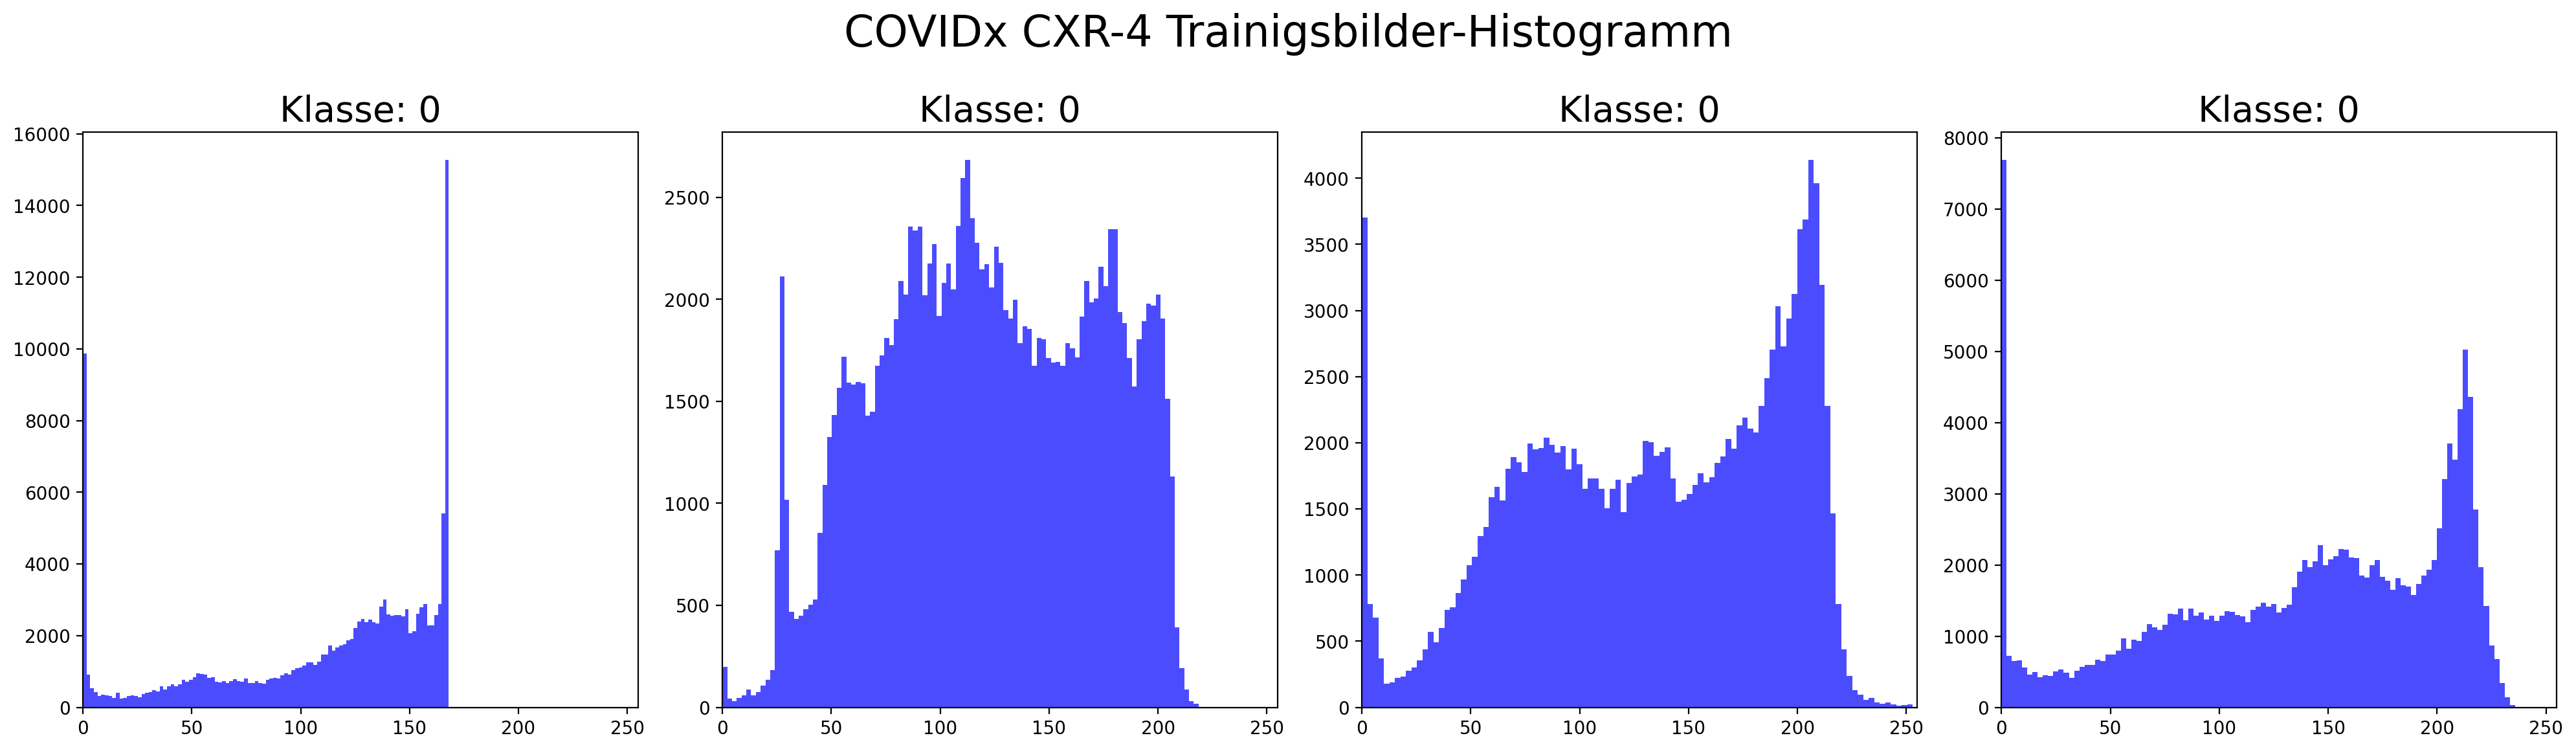
\includegraphics[width=\linewidth]{01-images/03-data/covid19-klasse0-hist.png}
    \caption{Histogramm der Pixelverteilung von den Bildern aus Abbildung \ref{fig:covid19-beispiele-klasse0-negativ} mit einer Bin-Grösse von 100}
    \label{fig:covid19-klasse0-hist}
\end{figure}

\begin{figure}[H]
    \centering
    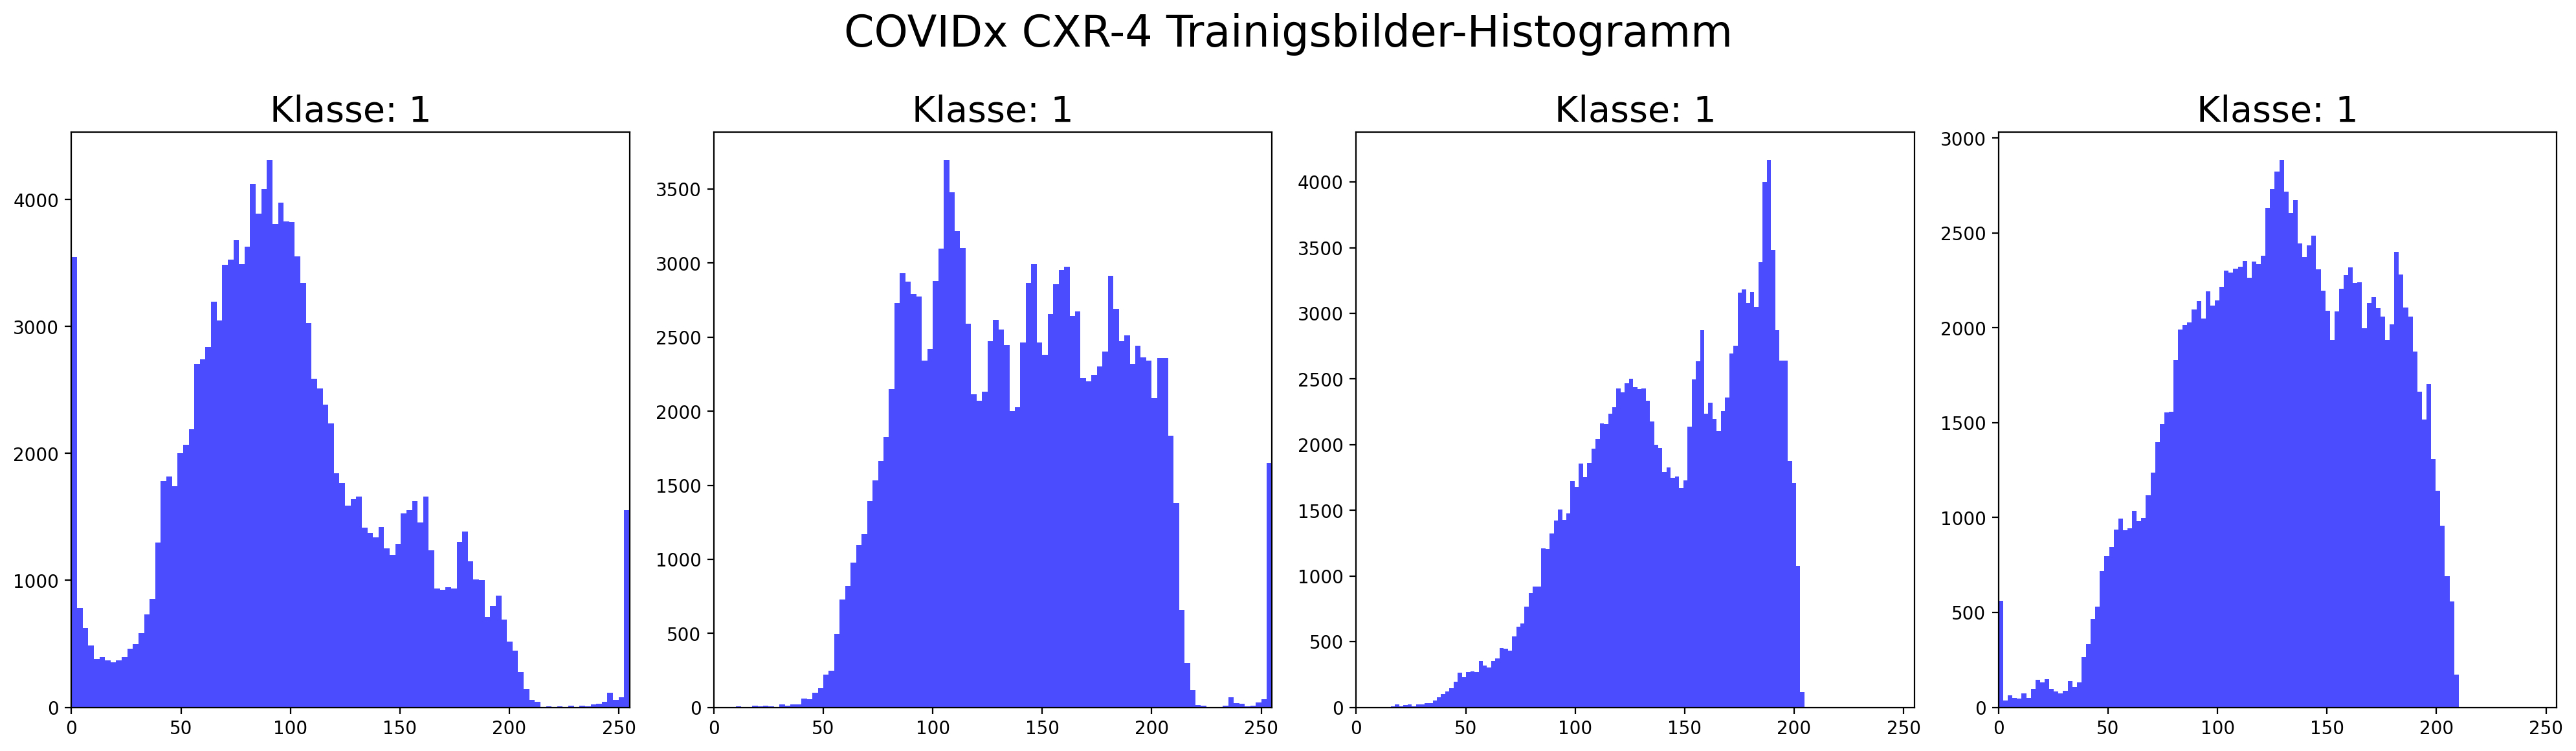
\includegraphics[width=\linewidth]{01-images/03-data/covid19-klasse1-hist.png}
    \caption{Histogramm der Pixelverteilung von den Bildern aus Abbildung \ref{fig:covid19-beispiele-klasse1-positiv} mit einer Bin-Grösse von 100}
    \label{fig:covid19-klasse1-hist}
\end{figure}

\subsubsection{Datenverteilung} \label{chap:COVID19-datenverteilung}
Im Verlauf dieser Thesis zeigte sich, dass die Performance Metriken der Testdaten von COVID-19 nicht den erwarteten Werten entsprachen. Daher wurde eine umfassende explorative Analyse der Trainings-, Validierungs- und Testdaten durchgeführt, um potenzielle Ursachen für diese Diskrepanzen zu identifizieren. In diesen Unterkapiteln werden die Ergebnisse dieser Untersuchungen festgehalten.

\paragraph{Pixelverteilung} \label{chap:COVID19-pixelverteilung}
Um die Verteilung der Pixelwerte zu analysieren, werden alle Bilder einer Partition zu einem eindimensionalen Vektor abgeflacht. Die resultierenden Vektoren werden mithilfe von Histogrammen visualisiert, wie in Abbildung \ref{fig:covid-datapartition-pixelverteilung-histo} dargestellt.

\begin{figure}[H]
    \centering
    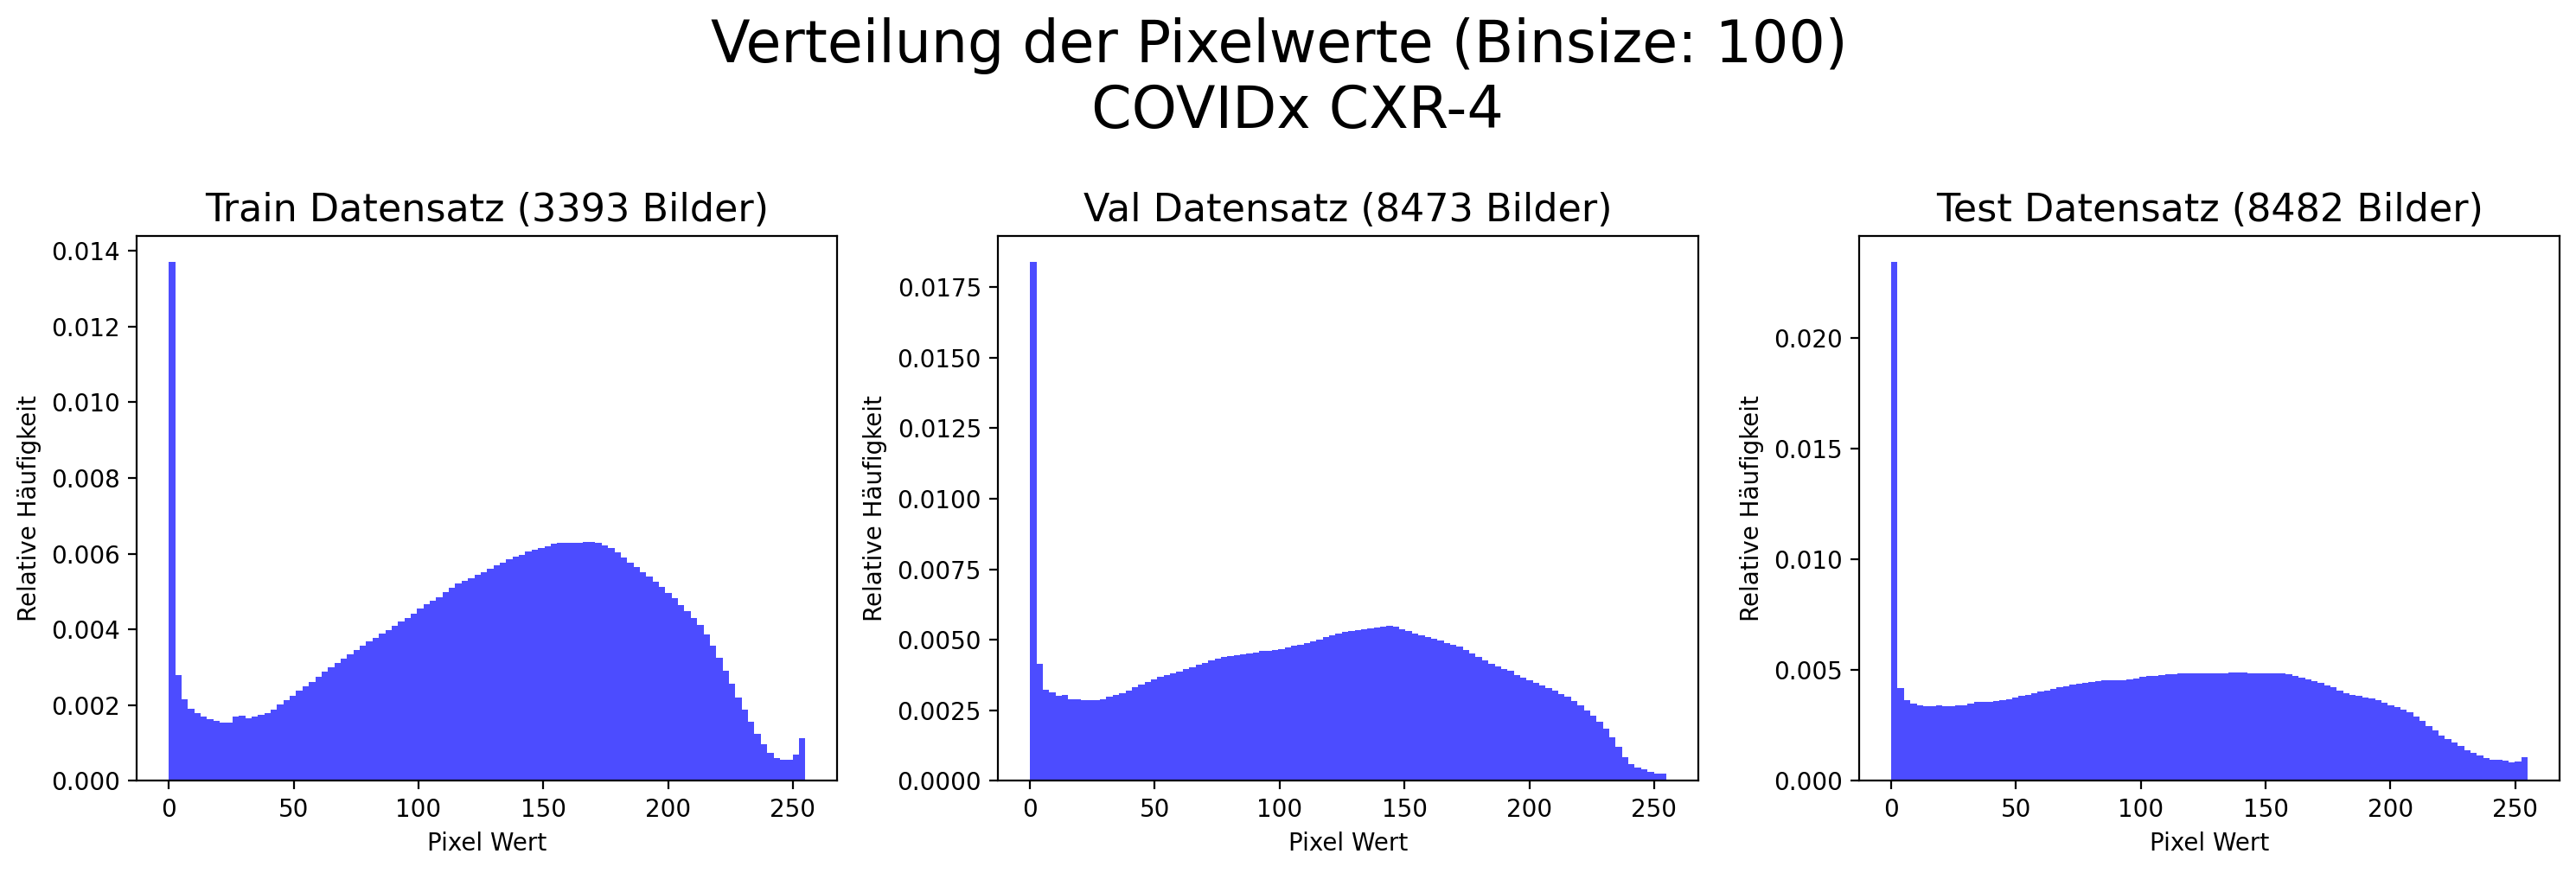
\includegraphics[width=\linewidth]{01-images/03-data/covid-Pixelverteilung-Partitionen.png}
    \caption{Histogramme der Pixelverteilung von jeder Datenpartition im COVIDx CXR-4 Datensatz}
    \label{fig:covid-datapartition-pixelverteilung-histo}
\end{figure}

Die Histogramme weisen charakteristische Merkmale von Röntgenaufnahmen auf, mit einer hohen Häufigkeit von Pixelwerten nahe null, die schwarzen Pixeln entsprechen. Ein markanter Gipfel bei einem Pixelwert von etwa 180 ist im Trainings- und, weniger ausgeprägt, im Validierungsdatensatz zu beobachten. Der Testdatensatz zeigt hingegen ein abweichendes Muster. Der typische Gipfel fehlt weitgehend, stattdessen ist ein leichter Anstieg am oberen Ende der Verteilung erkennbar, was auf einen höheren Anteil weisser Pixel hindeutet. 

Während die Pixelwertverteilungen in den Trainings- und Validierungsdaten trotz Intensitäts-unterschieden ähnliche Muster aufweisen, hebt sich der Testdatensatz deutlich ab. Diese Diskrepanz könnte auf verschiedene Faktoren zurückzuführen sein, wie unterschiedliche Bildaufnahmetechniken zwischen den Datenpartitionen, variierende Belichtungszeiten oder Sensoreinstellungen sowie den Einsatz verschiedener Röntgengeräte bei der Datenerfassung. Diese Beobachtungen legen nahe, dass der Testdatensatz möglicherweise einer anderen statistischen Verteilung folgt als die Trainings- und Validierungsdaten.

\paragraph{Pixelmittelwert} \label{chap:COVID19-pixelmittelwert}
Die folgende Visualisierung \ref{fig:covid-pixelmittelwert-comparison} dient dem Zweck, Unterschiede zwischen den Datenpartitionen anschaulich darzustellen und mögliche Auffälligkeiten oder Muster sichtbar zu machen. Für jede Datenpartitionen wurden Pixelmittelwerte berechnet, die den durchschnittlichen Pixelwert innerhalb einer festgelegten Dimension von 224 x 224 Pixeln repräsentieren. Diese spezifische Dimensionsgrösse wurde gewählt, da unsere Bilder beim Preprocessing auf diese Grösse reduziert werden.

\begin{figure}[H]
    \centering
    \begin{subfigure}[b]{0.49\linewidth}
        \centering
        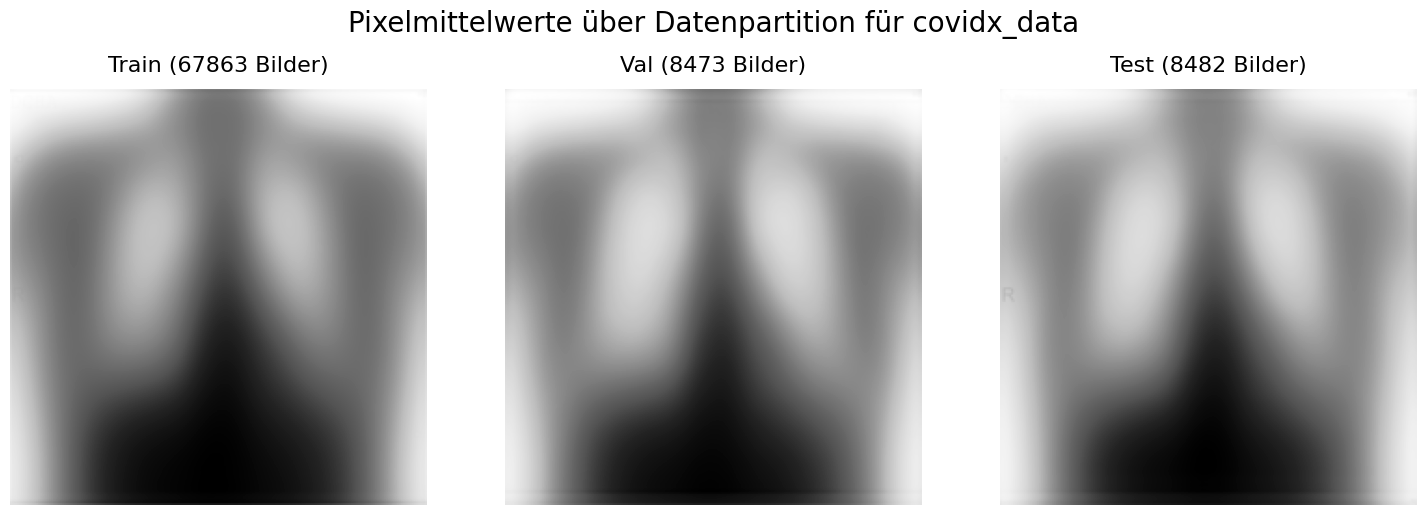
\includegraphics[width=\linewidth]{01-images/03-data/covid-pixelmittelwerte.png}
        \caption{Visuelle Darstellung der Pixelmittelwerte von aller COVID-19-Bildern pro Datenpartition}
        \label{fig:covid-pixelmittelwert-full}
    \end{subfigure}
    \hfill
    \begin{subfigure}[b]{0.49\linewidth}
        \centering
        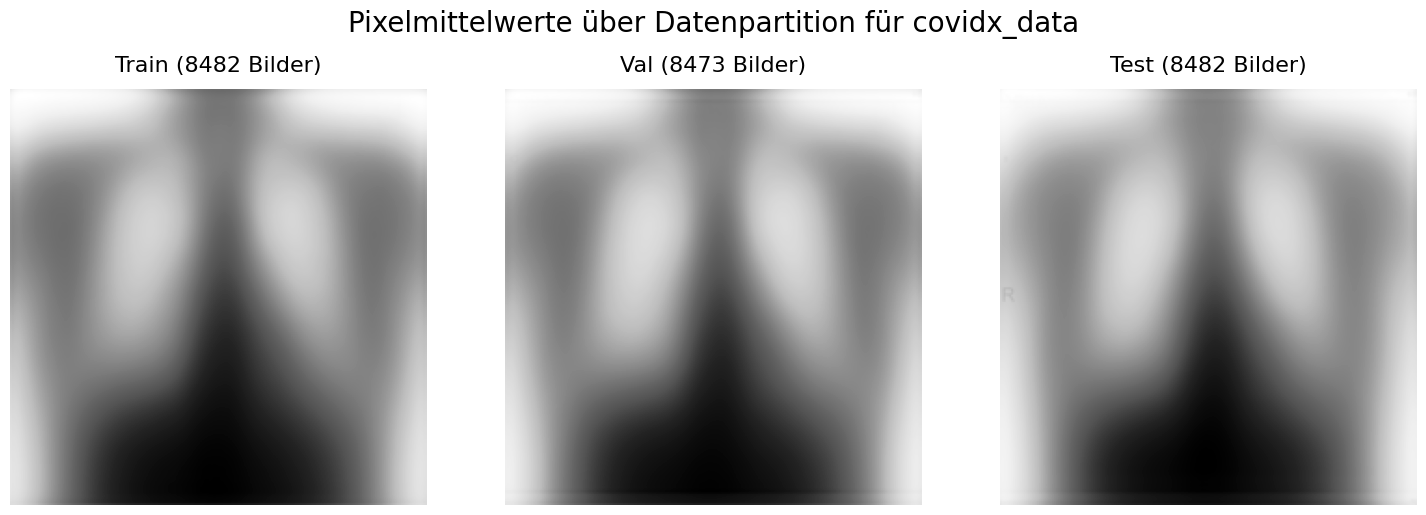
\includegraphics[width=\linewidth]{01-images/03-data/covidx-pixelmittelwert-subsample-train.png}
        \caption{Visuelle Darstellung der Pixelmittelwerte einer Teilmenge von COVID-19-Bildern Datenpartition}
        \label{fig:covid-pixelmittelwert-subsample}
    \end{subfigure}
    \caption{Vergleich der Pixelmittelwerte von COVID-19-Bildern}
    \label{fig:covid-pixelmittelwert-comparison}
\end{figure}

Die Analyse der Pixelmittelwerte über die verschiedenen Datenpartitionen des COVIDx CXR-4-Datensatzes zeigt minimale Unterschiede zwischen Trainings-, Validierungs- und Testpartitionen. In allen Datenpartitionen sind beide Lungenflügel sowie das umliegende Bauchgewebe deutlich erkennbar. Die Dunkelheit in der Mitte der Bilder könnte auf die Dichte des Gewebes in diesen Bereichen hindeuten, während hellere Bereiche weniger dichte Gewebe repräsentieren. Die Trainingspartition enthält wesentlich mehr Bilder als die Validierungs- und Testpartitionen. Daher wurde Abbildung \ref{fig:covid-pixelmittelwert-subsample} erstellt, die eine Teilmenge der Trainingsbilder zeigt. Visuell sind zwischen Abbildung \ref{fig:covid-pixelmittelwert-full} und \ref{fig:covid-pixelmittelwert-subsample} minimale Unterschiede zu erkennen.

\paragraph{Differenzbilder} \label{chap:COVID19-differenzbilder}
Eine weiterführende Analyse der Pixelmittelwerte wird durch die Berechnung der Differenzen zwischen den Datenpartitionen durchgeführt. Abbildung \ref{fig:differenz-datapartition-covid} visualisiert diese Unterschiede in Form einer Heatmap. Dabei werden die in Abbildung \ref{fig:covid-pixelmittelwert-full} dargestellten Pixelmittelwerte jeder Datenpartition voneinander subtrahiert, um die Differenzen anschaulich darzustellen.

\begin{figure}[H]
    \centering
    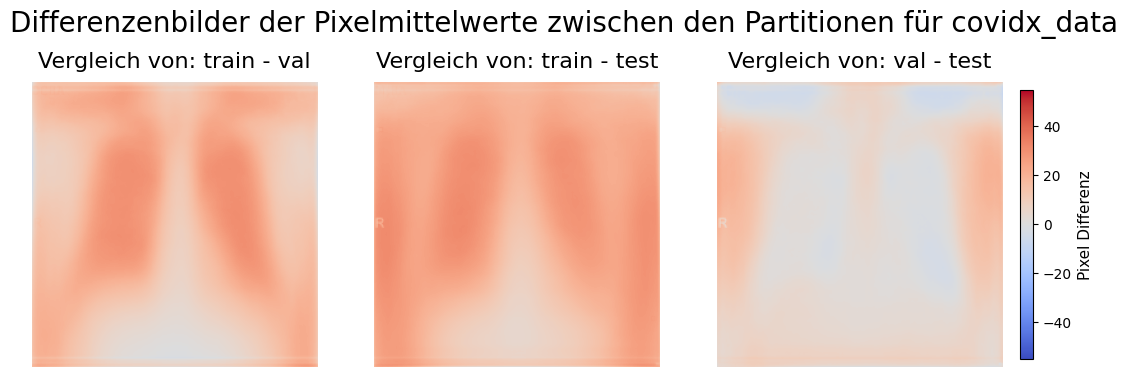
\includegraphics[width=\linewidth]{01-images/03-data/covidx-differenzenbilder.png}
    \caption{Differenzbilder von jeder Datenpartition aus Abbildung \ref{fig:covid-pixelmittelwert-full}}
    \label{fig:differenz-datapartition-covid}
\end{figure}

Der linke Abschnitt zeigt die Differenzen der durchschnittlichen Pixelwerte zwischen Trainings- und Validierungsdaten. Diese werden berechnet, indem die Mittelwerte der Validierungsdaten von denen der Trainingsdaten subtrahiert werden. Eine rote Färbung weist auf Regionen hin, in denen der Trainingsdatensatz höhere durchschnittliche Pixelwerte aufweist als der Validierungsdatensatz. Umgekehrt deutet eine blaue Färbung auf Bereiche, in denen die durchschnittlichen Pixelwerte im Trainingsdatensatz niedriger sind als im Validierungsdatensatz.

Im mittleren Abschnitt werden die Differenzen der durchschnittlichen Pixelwerte zwischen Trainings- und Testdaten visualisiert, berechnet durch Subtraktion der Testdaten von den Trainingsdaten. 

Im rechten Abschnitt werden die Differenzen der durchschnittlichen Pixelwerte zwischen Validierungs- und Testdaten visualisiert, berechnet durch Subtraktion der Testdaten von den Validierungsdaten.

Diese visuellen Darstellungen der Differenzen weisen auf potenzielle Verzerrungen und Ungleichgewichte zwischen den Datenpartitionen im COVIDx CXR-4 Datensatz hin, die sich auf die Modellleistung auswirken könnten. Besonders auffällig sind die Unterschiede zwischen dem Trainings- und den Validierungsdaten sowie zwischen dem Trainings- und den Testdaten, wobei die Diskrepanzen zwischen Trainings- und Testdaten am ausgeprägtesten erscheinen.

\newpage